\capitulo{4}{Técnicas y herramientas}
\section{Metodologías}

Como metodología para el desarrollo del proyecto se ha utilizado \textbf {Scrum}.
\emph{Scrum} es un marco de trabajo. Es el método ágil de desarrollo de Software más utilizado del mundo.
Entre sus características principales están:
utilizar una estrategia de desarrollo incremental, en lugar de la planificación y ejecución completa del producto. 
La calidad del resultado obtenido depende más del conocimiento tácito de las personas, que de la calidad de los procesos usados. 
Este método permite el solapamiento entre diferentes fases del proyecto.
Algunos de sus componentes principales son: 
\begin{itemize}
\item\textbf{Sprint:} Parte básica en este tipo de desarrollos, donde se desarrolla un incremento del producto que pueda ser utilizado.
\item\textbf{Pila del producto:} donde están los requisitos de usuario, esta información no es rígida, puede variar según va evolucionando el producto.
\item\textbf{Pila del \emph{sprint}:} lista con las tareas a realizar durante un \english{sprint}.
\item{Incremento:} Parte del desarrollo obtenida al final de cada \english{sprint}.
\end{itemize}
Durante todo el proyecto se han ido realizando los diferentes \english{sprints}, en los cuales se han planificado las tareas siguientes y revisado, si se han ido cumpliendo los objetivos marcados en el \english{sprint} anterior.


\section{Patrones de diseño}
\emph{Flask} utiliza como patrón de diseño, \textbf {MTV}.
El patrón \emph{MTV} es similar al conocido \emph{MVC}, pero con algunas diferencias:

En el patrón \emph{MVC}:
\begin{itemize}
\item\textbf{Modelo:} Es la parte que manipula la información.
\item\textbf{Vista:} Decide como se mostrará la información.
\item\textbf{Controlador:} Comunica el modelo con la vista.
\end{itemize}
Podemos ver a continuación sus equivalencias, para este caso, usando el \english{framework} \texttt{Flask}:

\begin{table}[!h]
\centering
\begin{tabular}{lr}
\toprule
\textbf{MVC}& \multicolumn{1}{r}{\textbf{MTV}} \\ 
\midrule
Modelo & Modelo\\
Vista & Vista y Template\\
Controlador & \texttt{Flask} \\ 
\bottomrule
\end{tabular}
\caption{MVC vs MTV.}
\label{stats}
\end{table}


Aquí, el \emph{framework} \texttt{Flask}, es el que toma el papel del controlador.
Resumiendo, en el patrón \emph{MTV}, tenemos:
\begin{itemize}
\item\textbf{Modelo:} Es la parte que manipula la información, se encuentra en forma de clases de Python.
\item\textbf{Vista:} Decide qué información se muestra y en que \english{template}.
\item\textbf{Template:} Coge toda la información, la organiza y ve la manera en que esta se va a mostrar. Básicamente una página \emph{HTML} con algunas etiquetas extras propias de \emph{Jinja2} el motor de plantillas utilizado por defecto por \texttt{Flask}.
\end{itemize}

\imagen{MTV}{Esquema de un patrón \emph{MTV}}

En la imagen anterior podemos ver como son las relaciones en el patrón \emph{MTV}:
\begin{enumerate}
\item El Navegador manda una solicitud 
\item La vista interactúa con el modelo para obtener datos. 
\item La vista llama a la plantilla. 
\item La plantilla renderiza la respuesta a la solicitud del navegador 
\end{enumerate}

\section{Control de Versiones}

Existen varias herramientas en el mercado para el control de versiones:
\begin{itemize}
\item\textbf{Git}\footnote{\textsl{Git}: \url{https://git-scm.com/}}
\item \textbf{Subversion}\footnote{\textsl{Subversion}: \url{https://subversion.apache.org/}}
\item \textbf{SourceSafe}\footnote{\textsl{SourceSafe}: \url{https://es.wikipedia.org/wiki/Microsoft_Visual_SourceSafe}}
\end{itemize}

Nos hemos decantado por \textbf {Git}, ya que es la que se ha venido usando durante la realización del grado y es una de las mas extendidas en el mercado.

\emph{Git} es un sistema de control de versiones distribuido, libre y de código abierto. \emph{Git} se distribuye bajo la licencia de software libre GNU LGPL v2.1. 

\section{Hosting del repositorio}

Al igual que en el apartado anterior, aunque existen diversas posibilidades:
\begin{itemize}
\item \textbf{GitLab}\footnote{\textsl{GitLab}: \url{https://about.gitlab.com/}}
\item \textbf{GitHub}\footnote{\textsl{GitHub}: \url{https://github.com/}}
\item \textbf{Bitbucket}\footnote{\textsl{Bitbucket}: \url{https://bitbucket.org/}}
\end{itemize}

Como en el apartado anterior, por familiaridad con la plataforma durante el grado y también por ser una de las más usadas, de decidió usar \textbf {GitHub}.

\emph{GitHub} permite tener cuentas gratuitas y de pago. Además, un tipo de cuenta para estudiantes, como alumno se puede solicitar acogerte al programa <<\english{GitHub education for students}>>, que te permite tener repositorios privadas y da acceso a herramientas adicionales.

Además, \emph{GitHub} ofrece otras funcionalidades y servicios como, por ejemplo; revisión de código, documentación, gestión de tareas, \english{wikis} e integraciones con otros servicios como por ejemplo \emph{CodeBeat}.

\section{Gestión del proyecto}

Dentro de las muchas herramientas existentes como por ejemplo;
\begin{itemize}
\item \textbf{ZenHub}\footnote{\textsl{ZenHub}: \url{https://www.zenhub.com/}}
\item \textbf{Trello}\footnote{\textsl{Trello}: \url{https://trello.com/}}
\item \textbf{VersionOn}\footnote{\textsl{VersionOne}: \url{https://www.collab.net/}}
\end{itemize}

Se ha optado por usar  \textbf {ZenHub} ya que se encuentra integrado en el propio \emph{GitHub}, funciona como una aplicación nativa en su interfaz y podemos controlar nuestros proyectos usando paneles de trabajo bastante intuitivos, así como conectar con varios repositorios en el panel de tareas y ver todos los temas abiertos que requieren de la atención.

Se trata de una plataforma de gestión de proyectos de software y entre las principales características de ZenHub están la de convertir los \english{issues} de \emph{GitHub} en dinámicos tablones \emph{Kanban}.

\section{Entorno de desarrollo integrado (IDE)}


\subsubsection{Python}

Como en los apartados anteriores se han tenido en cuenta diferentes herramientas para este trabajo:
\begin{itemize}
\item \textbf{NotePad ++}\footnote{\textsl{NotePad ++}: \url{https://notepad-plus-plus.org/}}
\item \textbf{Sublime Text}\footnote{\textsl{Sublime Text}: \url{https://www.sublimetext.com/}}
\item \textbf{Microsoft Visual Studio Code}\footnote{\textsl{Microsoft Visual Studio Code}: \url{https://code.visualstudio.com/}}
\item \textbf{PyCharm}\footnote{\textsl{PyCharm}: \url{https://www.jetbrains.com/pycharm/}}

\end{itemize}

Tanto \emph{Microsoft Visual Studio Code} como \emph{PyCharm} son perfectamente válidas y las más completas para realizar este tipo de proyectos, abarcan casi todos los lenguajes de programación, contienen bastantes \english{plugins} y facilitan el trabajo a la hora de realizar los test.

Al final nos hemos decantado por \textbf{PyCharm}. Al haberse realizado el proyecto con Python, este entorno ha sido diseñado para este lenguaje, por lo que ofrece algunas ventajas más, respecto a \emph{Microsoft Visual Studio Code}. \emph{PyCharm} es soportado por Windows, Mac OS y Linux, y su versión gratuita es bastante completa. Existen también licencias individuales para estudiantes.



\subsubsection{\LaTeX}
La documentación del proyecto ha desarrollado en \LaTeX. Para este propósito se han tenido en cuenta las siguientes herramientas:
\begin{itemize}
\item \textbf{MikTex}\footnote{\textsl{MikTex}: \url{https://miktex.org/}}, para SO Windows.
\item \textbf{texlive}\footnote{\textsl{texlive}: \url{https://www.tug.org/texlive/}}, para SO Linux.
\item \textbf{MacTex}\footnote{\textsl{MacTex}: \url{http://www.tug.org/mactex/}}, para SO Mac.
\item \textbf{Texmaker}\footnote{\textsl{Texmaker}: \url{http://www.xm1math.net/texmaker/}}, compatible con las 3 plataformas.
\item \textbf{Overleaf}\footnote{\textsl{Overleaf}: \url{ https://es.overleaf.com/}}, editor en línea.
\end{itemize}

Se ha optado por \textbf{Texmaker} como editor y \textbf{MikTex} como distibución de \LaTeX, recomendadas por el tutor del proyecto.
Integran la mayoría de herramientas necesarias para la escritura de documentos en \LaTeX, es gratuito y tiene licencia GNU GPL v2.

\section{Servicios de integración continua}


\subsubsection{Calidad del código}
Las diferentes herramientas consideradas para este propósito han sido: 
\begin{itemize}
\item \textbf{SonarQube}\footnote{\textsl{SonarQube}: \url{https://www.sonarqube.org/}}
\item \textbf{CodeBeat}\footnote{\textsl{CodeBeat}: \url{https://codebeat.co/}}
\end{itemize}

Se ha optado por \textbf{CodeBeat}, ya que se integra perfectamente con \emph{GitHub}. Es una herramienta gratuita, que soporta gran cantidad de lenguajes y permite personalizar totalmente, las métricas que usa para el análisis de la calidad del código.

\section{Herramienta de análisis sintáctico}

Como herramienta de análisis sintáctico, para poder dar validez a los archivos de entrada, se pensó en estas 3 posibilidades:
\begin{itemize}
\item \textbf{Ply}\footnote{\textsl{Ply}: \url{https://pypi.org/project/ply/}}
\item \textbf{Antlr}\footnote{\textsl{Antlr}: \url{https://www.antlr.org/}}
\item \textbf{Flex Bison}\footnote{\textsl{Flex Bison}: \url{https://www.oreilly.com/library/view/flex-bison/9780596805418/}}
\end{itemize}

La opción elegida ha sido \textbf{Ply}, ya que está implementada completamente en Python y encaja perfectamente con la filosofía de realizar la mayor parte del proyecto con este lenguaje.

Aunque \texttt{\texttt{Ply}} también es una biblioteca y debería estar en el apartado de bibliotecas, le hemos querido dar un apartado especial como herramienta de análisis sintáctico.

\texttt{Ply} es una biblioteca de Python. Es una implementación de lex y yacc de herramientas de análisis para Python, que proporciona la mayor parte de las características estándar de \texttt{lex / yacc}, incluyendo; el apoyo a las producciones vacías, las reglas de prioridad, la recuperación de errores y soporte para gramáticas ambiguas. Si se tiene experiencia previa con alguna herramienta de generación de analizadores sintácticos, es muy sencillo de usar, y también muy efectivo a la hora de realizar la comprobación de los errores. \texttt{Ply} utiliza el análisis \texttt{LR}, el cual puede incorporar grandes gramáticas fácilmente.

\texttt{Ply}, básicamente está compuesto de 2 módulos:
\begin{itemize}
\item \texttt{ply.lex} – Donde se trata la parte del análisis léxico
\item \texttt{ply.yacc} -  Este módulo es para crear un \english{parser}.
\end{itemize}

\section{Bibliotecas}

A continuación, vemos el resto de las bibliotecas necesarias en el desarrollo de este proyecto:


\subsubsection{ezdxf}

\texttt{ezdxf}\footnote{\textsl{ezdxf}: \url{ https://ezdxf.readthedocs.io}} es la biblioteca más importante del proyecto. En un principio, se tuvieron en cuenta otras opciones como:
\begin{itemize}
\item \textbf{dxfgrabber}\footnote{\textsl{dxfgrabber}: \url{https://pypi.org/project/dxfgrabber/}}
\item \textbf{SDXF}\footnote{\textsl{SDXF}: \url{https://pypi.org/project/SDXF/}}
\item \textbf{dxfwrite}\footnote{\textsl{dxfwrite}: \url{https://pypi.org/project/dxfwrite/}}
\end{itemize}

Resultando la opción más interesante \texttt{ezdxf}, ya que era la única que cubría todas las necesidades que aquí se planteaban.

\texttt{ezdxf} es una interfaz de Python para el formato DXF, desarrollado por \emph{Autodesk}, y que permite a los desarrolladores leer y modificar dibujos DXF existentes o crear nuevos dibujos DXF.

Con sus métodos y atributos nos permite crear, modificar, eliminar o consultar las propiedades de todos los elementos que puede contener un archivo de CAD.
\texttt{ezdxf} es independiente del sistema operativo y se ejecuta en todas las plataformas que proporcionan un intérprete de Python adecuado (> = 3.6). Está bajo la licencia MIT-License.

Una parte a destacar, es que nos permite generar el DXF en distintas versiones de un archivo CAD, lo cual es muy interesante. 


\begin{figure}[!h]
	\centering
	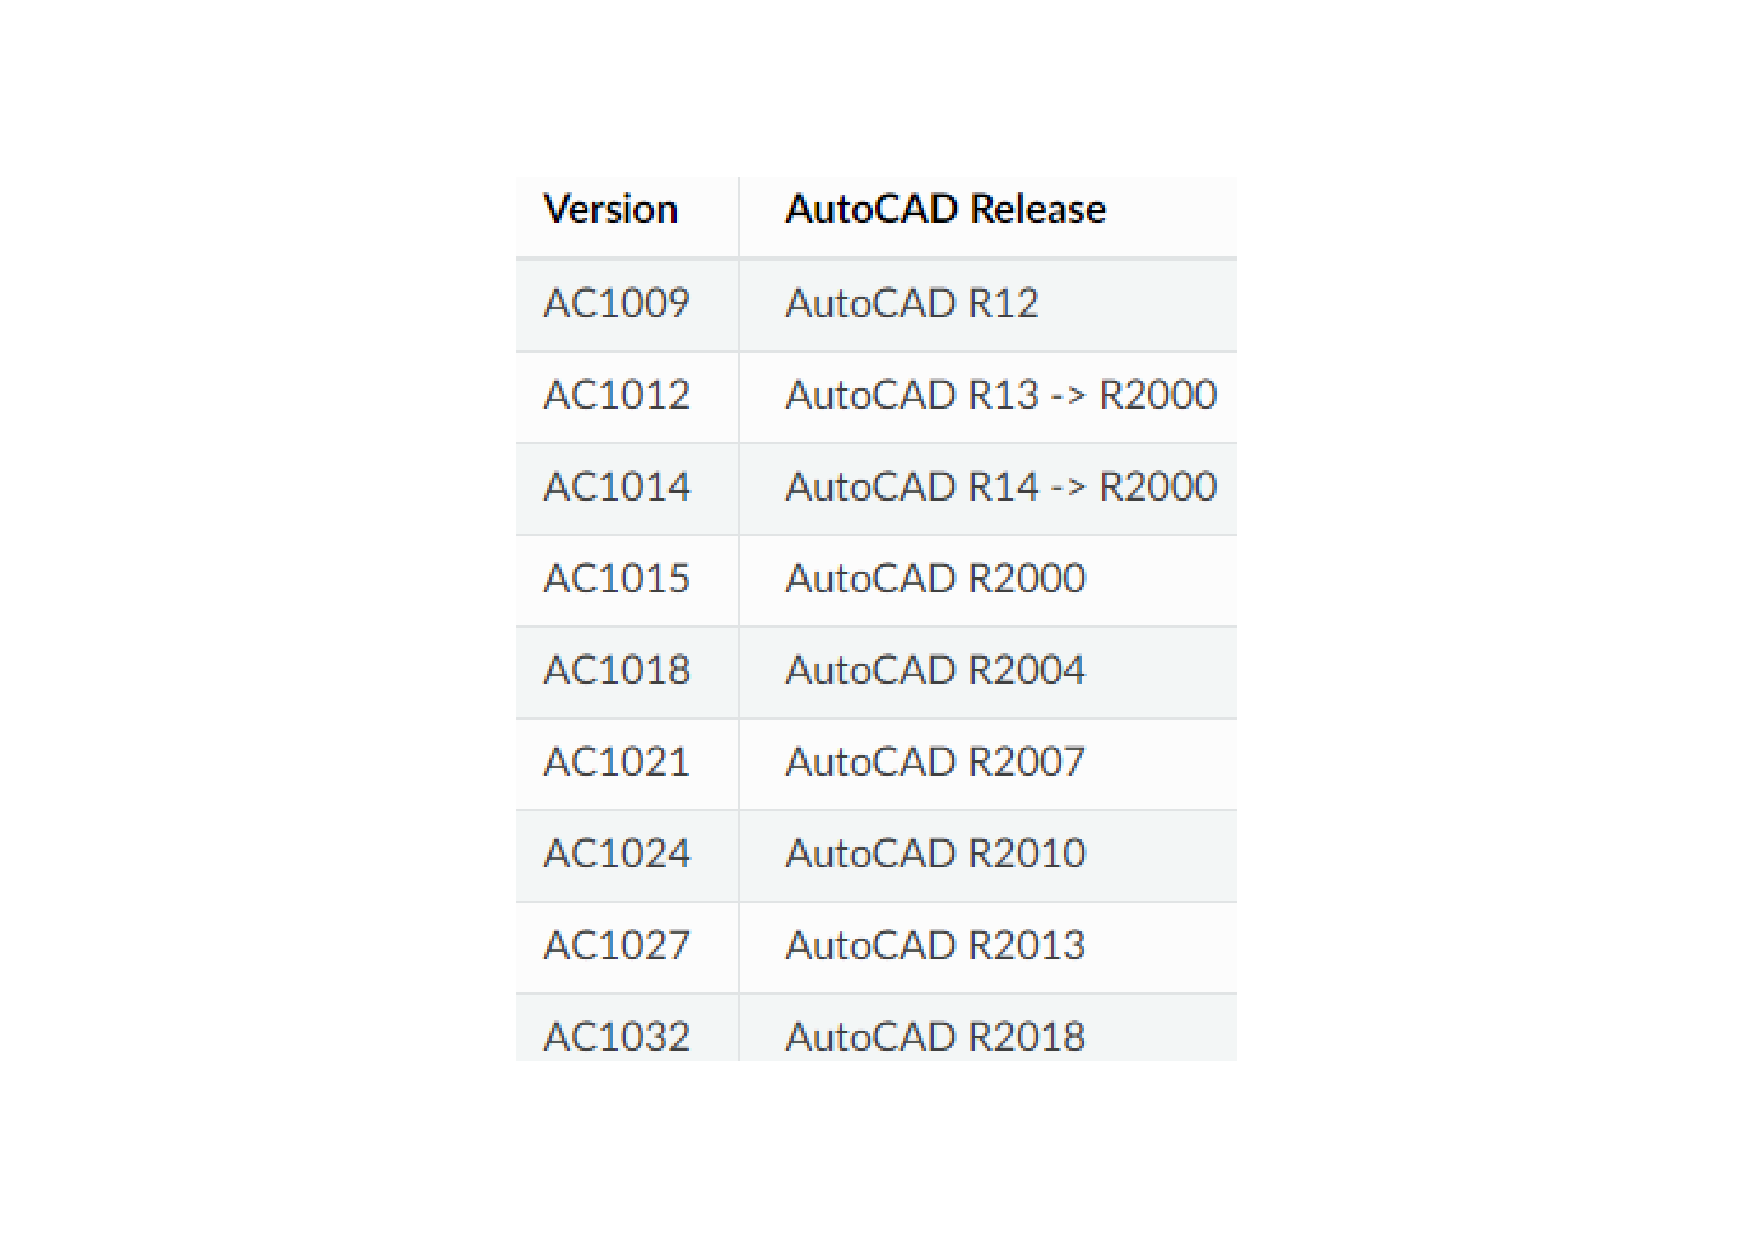
\includegraphics[width=0.4\textwidth]{Cad_versions}
	\caption{Versiones de CAD.}
	\label{fig:Cad_versions}
\end{figure}

\subsubsection{SQLAlchemy}
Las diferentes herramientas consideradas para este propósito han sido:

\begin{itemize}
\item \textbf{peewee}\footnote{\textsl{peewee}: \url{http://docs.peewee-orm.com}}
\item \textbf{SQLAlchemy}\footnote{\textsl{SQLAlchemy}: \url{https://www.sqlalchemy.org/}}
\end{itemize}
Se ha elegido la biblioteca de Python \textbf{SQLAlchemy}, a pesar de ser algo más complejo que \emph{peewee}, al ser más utilizado, es más fácil encontrar información cuando se presenta un problema de funcionamiento.

\subsubsection{Flask-Login}
Las diferentes herramientas consideradas para este propósito han sido:

\begin{itemize}
\item \textbf{Flask-User}\footnote{\textsl{Flask-User}: \url{https://flask-user.readthedocs.io/en/latest/}}
\item \textbf{Flask-Security}\footnote{\textsl{Flask-Security}: \url{https://pythonhosted.org/Flask-Security/}}
\item \textbf{Flask-Login}\footnote{\textsl{Flask-Login}: \url{https://flask-login.readthedocs.io/en/latest/}}
\end{itemize}

Se ha elegido la biblioteca de Python \textbf{Flask-Login}, ofrece todo lo necesario y es la utilizada en la mayoría de los ejemplos de autentificación de usuarios con \texttt{Flask}.

\subsubsection{Bootstrap}
Los diferentes \english{frameworks} CSS consideradas para este propósito han sido:

\begin{itemize}
\item \textbf{Bootstrap}\footnote{\textsl{Bootstrap}: \url{https://getbootstrap.com/}}
\item \textbf{Foundation}\footnote{\textsl{Foundation}: \url{https://foundation.zurb.com/}}
\item \textbf{Materialize}\footnote{\textsl{Materialize}: \url{https://materializecss.com/}}
\end{itemize}

Se ha elegido \textbf{Bootstrap}, es  el \english{framework} de uso más extendido, y como consecuencia con mejor soporte a la hora de hacer búsquedas para resolver problemas.Es un english{framework} Open Source.


\subsubsection{Colorpicker Bootstrap}

\textbf{Colorpicker Bootstrap}, es un \english{plugin} de selector de color modular para\emph{ Bootstrap 4}. Está bajo la licencia MIT-License.


\subsubsection{TinyColor}

Es un micro \english{framework} que permite la manipulación y conversión de color en \emph{JavaScript}. Permite muchas formas de entrada, mientras que proporciona conversiones de color y otras funciones de utilidad de color. No tiene dependencias. Está bajo la licencia MIT-License.


\subsubsection{bs-custom-file-input}

\textbf{bs-custom-file-input}, es un \english{plugin} para \emph{Bootstrap 4}. Ayuda a crear una entrada de selección de archivos personalizada con el botón del navegador para cargar archivos. También es compatible con múltiples selecciones de archivos y arrastrar y soltar.
No tiene dependencias. Está bajo la licencia MIT-License.

\subsubsection{jquery.cookie}

\textbf{jquery.cookie}, es un es un \english{plugin} de  \english{jQuery}, para trabajar con \emph{cookies}.
No tiene dependencias. Está bajo la licencia MIT-License.



\section{Desarrollo Web}

Para el desarrollo web, del lado del servidor, se ha optado por utilizar \textbf{Flask}, siguiendo, como se ha comentado anteriormente con la idea de englobar lo máximo posible en Python.
\texttt{Flask} es un \english{micro framework} escrito en Python y concebido para facilitar el desarrollo de aplicaciones Web bajo el patrón MTV.

Entre algunas de sus ventajas, están:
\begin{itemize}
\item Desarrollo de aplicaciones web de una forma ágil y rápida, tiene una buena curva de aprendizaje
\item En desarrollo no se necesita una infraestructura con un servidor web.
\item Compatible con \emph{wsgi}.
\item Soporta de manera nativa el uso de \english{cookies} seguras.
\item Se pueden usar sesiones.
\item \texttt{Flask} es Open Source y tiene una licencia BSD.
\item Extensa documentación.
\end{itemize}

\section{Base de Datos: PostGIS}\label{sec:postgis}

Como sistema de base de datos se ha decidido utilizar \textbf{PostGIS}. \emph{PostGIS} convierte al sistema de administración de bases de datos \textbf{PostgreSQL} en una base de datos espacial mediante la adición de tres características: tipos de datos espaciales, índices espaciales y funciones que operan sobre ellos.

Puede parecer en un principio, que el uso de esta base de datos no está justificada en este proyecto, ya que de momento solo sirve para gestionar a los usuarios de la aplicación. Habitualmente trabajo con bases de datos espaciales y \emph{PostGIS} es la más usada en en el campo de los sistemas de información geográfica. A parte de poder usarla en desarrollos particulares, como este, programas de GIS como \emph{QGis, gvSIG o ArcGis}, que son aplicaciones de escritorio,  permiten una conexión directa con \emph{PostGIS}. 
La idea es que en un futuro ese contenedor pueda almacenar bases de datos espaciales, de otras aplicaciones de futuros desarrollos o de las que uso habitualmente. Ya que la vamos a tener en un contenedor \emph{Docker} con una base de datos alojada en él, darle el máximo uso en el futuro.

En España casi todas las instituciones que trabajan con datos geoespaciales, trabajan con \emph{PostGIS}, es una buena oportunidad para familiarizarse con ella.

La aplicación \textbf{SurveyingPointCode}, en un futuro, aumentará sus funcionalidades y para ello será necesario trabajar con \emph{PostGIS}.

\section{Despliegue de la aplicación}

Para el despliegue de la aplicación se ha optado por utilizar \textbf{Docker}. Principalmente, porque es una herramienta de mucha actualidad y con un gran potencial, tanto en el desarrollo, como en el despliegue de aplicaciones.

La idea básica de su funcionamiento es la creación de una serie de contenedores muy ligeros y portables, así las aplicaciones, podrán ejecutarse en cualquier equipo, solamente con tener \emph{Docker} instalado, con independencia del sistema operativo.

Entre algunas de sus ventajas, están:

\begin{itemize}
\item Es muy sencillo de usar.
\item Ahorra tiempo, no necesitamos instalar diferentes programas.
\item Los contenedores son muy ligeros, a diferencia de las máquinas virtuales, ya que no necesitan un sistema operativo completo, cogen lo que necesitan de cada máquina anfitriona.
\item Portabilidad.
\item Los repositorios \emph{Docker}, permiten acceder a gran cantidad de imágenes y así poder de ejecutar prácticamente todas las aplicaciones.
\item Es un entorno seguro y no ofrece variaciones, da igual cual sea el equipo ni el ambiente. Facilita las pruebas, el desarrollo y las visualizaciones por parte del cliente.
\item Es Open Source.
\item Extensa documentación.
\end{itemize}
